\documentclass[12pt,a4paper]{article}
\usepackage[utf8]{inputenc}
\usepackage[spanish]{babel}
\usepackage{graphicx}
\usepackage{amsmath}
\usepackage{amsfonts}
\usepackage{booktabs}
\usepackage{hyperref}
\usepackage{geometry}
\usepackage{float}
\usepackage{caption}
\usepackage{subcaption}
\usepackage{enumitem}
\usepackage{listings}
\usepackage{xcolor}
\geometry{margin=2.5cm}

\definecolor{codegreen}{rgb}{0,0.6,0}
\definecolor{codegray}{rgb}{0.5,0.5,0.5}
\lstset{
  basicstyle=\ttfamily\small,
  breaklines=true,
  frame=single,
  numbers=left,
  numberstyle=\tiny\color{codegray},
}

\title{\textbf{Laboratorio 6: DBSCAN + KDTree}\\ 
       \large Implementación y Comparación de Algoritmos de Clustering}
\author{Fabricio Messa}
\date{Junio 2025}

\begin{document}
\maketitle
\tableofcontents
\newpage

% ========================
\section{Introducción}
% ========================

El presente laboratorio tiene como objetivo implementar el algoritmo de clustering \textbf{DBSCAN} (Density-Based Spatial Clustering of Applications with Noise) en dos versiones: la implementación clásica con búsqueda de vecinos por fuerza bruta $O(n^2)$ y una versión optimizada utilizando un \textbf{KDTree} para la búsqueda de vecinos por radio.

Ambas implementaciones se realizan en \textbf{C++} y se comparan en términos de tiempo de ejecución sobre datasets sintéticos de 2 y 6 dimensiones. Las visualizaciones y métricas de evaluación (Silhouette Score) se generan mediante scripts en Python utilizando PCA y t-SNE para reducción de dimensionalidad.

% ========================
\section{Metodología}
% ========================

\subsection{Datasets}
Se generaron dos datasets sintéticos utilizando \texttt{sklearn.datasets.make\_blobs}:

\begin{itemize}
    \item \textbf{Dataset 2D:} 790 puntos, 2 dimensiones. Compuesto por 3 clusters gaussianos (250 puntos cada uno) con centros en $(2,2)$, $(8,3)$ y $(5,9)$, más 40 puntos de ruido uniforme.
    \item \textbf{Dataset 6D:} 850 puntos, 6 dimensiones. Compuesto por 4 clusters gaussianos (200 puntos cada uno) más 50 puntos de ruido uniforme.
\end{itemize}

\subsection{Algoritmo DBSCAN}
DBSCAN clasifica puntos como \textit{core}, \textit{border} o \textit{noise} basándose en dos hiperparámetros:

\begin{itemize}
    \item \texttt{eps} ($\varepsilon$): Radio máximo de vecindad.
    \item \texttt{min\_samples}: Número mínimo de puntos para considerar un punto como \textit{core}.
\end{itemize}

El algoritmo itera sobre los puntos no visitados, y si un punto tiene al menos \texttt{min\_samples} vecinos dentro del radio $\varepsilon$, inicia un nuevo cluster y lo expande recursivamente a todos los puntos alcanzables por densidad.

\subsection{Integración con KDTree}
En la versión clásica, la búsqueda de vecinos (\texttt{rangeQuery}) requiere $O(n)$ por punto, resultando en $O(n^2)$ total. Con KDTree, se construye un árbol balanceado en $O(n \log n)$ y cada búsqueda por radio se realiza en $O(\log n)$ en promedio para dimensiones bajas, reduciendo la complejidad total a $O(n \log n)$.

El KDTree implementado divide recursivamente el espacio en la mediana de cada dimensión, alternando la dimensión de partición por nivel. La búsqueda por radio poda ramas cuya distancia mínima al hiperplano de partición excede el radio de búsqueda.

% ========================
\section{Resultados}
% ========================

\subsection{Comparación de Tiempos de Ejecución}

\begin{table}[H]
\centering
\caption{Tiempos de ejecución (ms) para diferentes configuraciones}
\begin{tabular}{cccccc}
\toprule
\textbf{Dataset} & \textbf{eps} & \textbf{min\_samples} & \textbf{Clásico (ms)} & \textbf{KDTree (ms)} & \textbf{Speedup} \\
\midrule
2D & 1.5 & 5  & 2.90 & 2.83 & 1.02$\times$ \\
2D & 1.2 & 3  & 2.22 & 1.63 & 1.36$\times$ \\
2D & 1.8 & 3  & 1.61 & 1.50 & 1.07$\times$ \\
\midrule
6D & 4.0 & 10 & 3.53 & 2.65 & 1.33$\times$ \\
6D & 3.0 & 5  & 3.32 & 2.44 & 1.36$\times$ \\
6D & 5.0 & 15 & 2.67 & 2.15 & 1.24$\times$ \\
\bottomrule
\end{tabular}
\end{table}

El KDTree ofrece una mejora de velocidad del \textbf{24\%--36\%} en el dataset 6D y \textbf{2\%--36\%} en 2D. La mejora es más notoria en datasets de mayor dimensionalidad con más puntos, aunque la ventaja se reduce a medida que la dimensionalidad crece.

\begin{figure}[H]
\centering
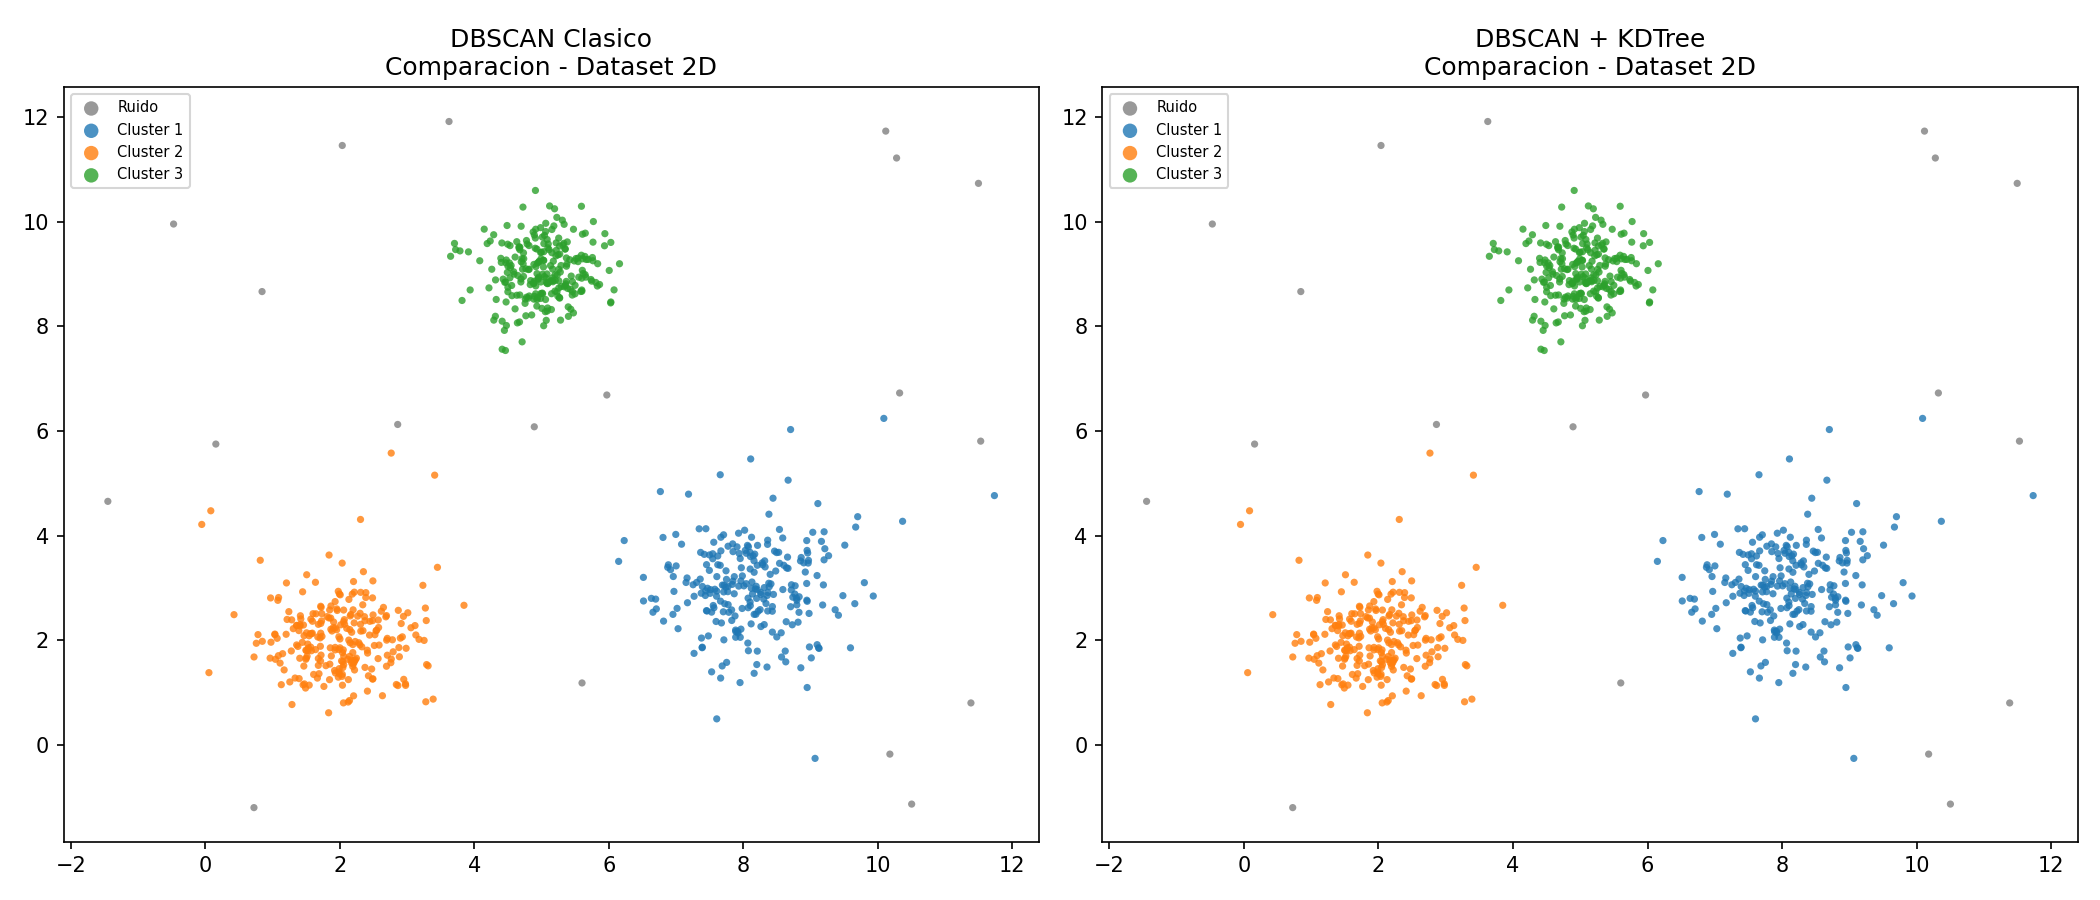
\includegraphics[width=0.9\textwidth]{resultados/comparison_2d_2d.png}
\caption{Comparación de clusters: DBSCAN Clásico vs DBSCAN + KDTree (2D, $\varepsilon=1.5$, minPts=5)}
\end{figure}

\subsection{Análisis con Diferentes Hiperparámetros}

\begin{figure}[H]
\centering
\begin{subfigure}{0.48\textwidth}
    \centering
    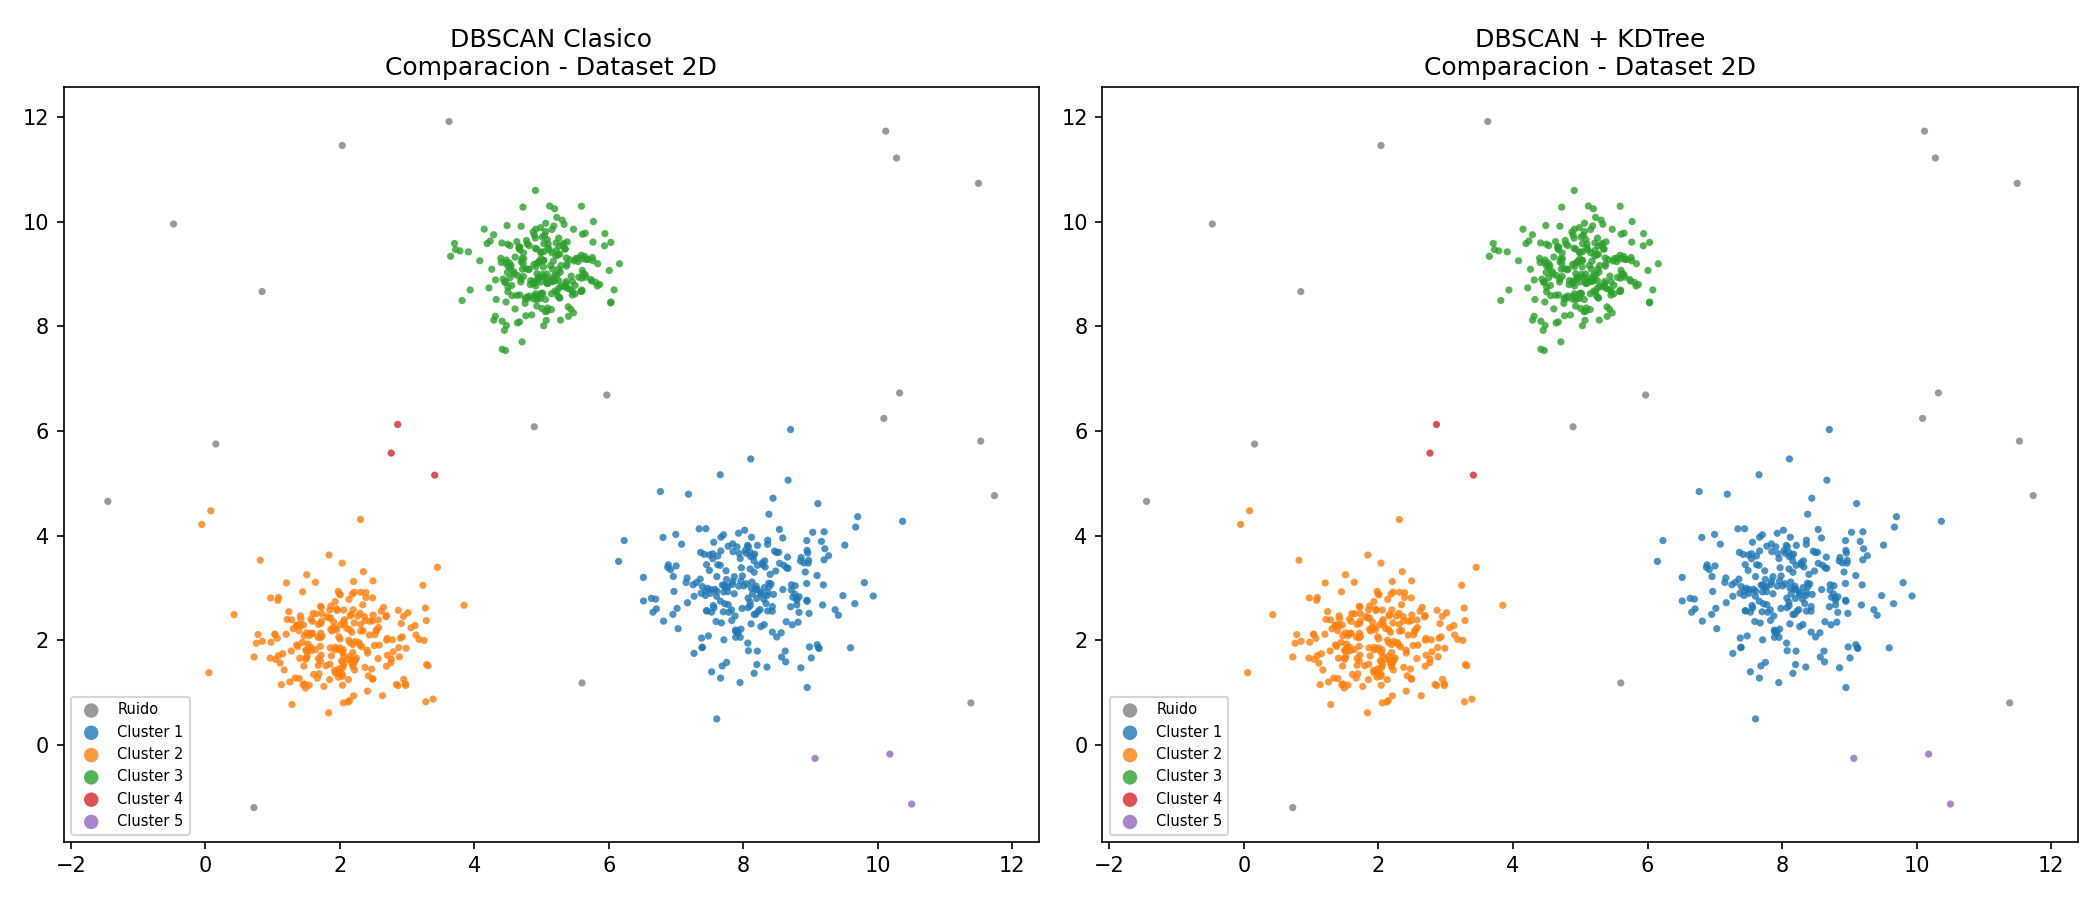
\includegraphics[width=\textwidth]{resultados/comparison_2d_2d_eps1.2_mp3.png}
    \caption{$\varepsilon=1.2$, minPts=3 (sobre-clusterización)}
\end{subfigure}
\hfill
\begin{subfigure}{0.48\textwidth}
    \centering
    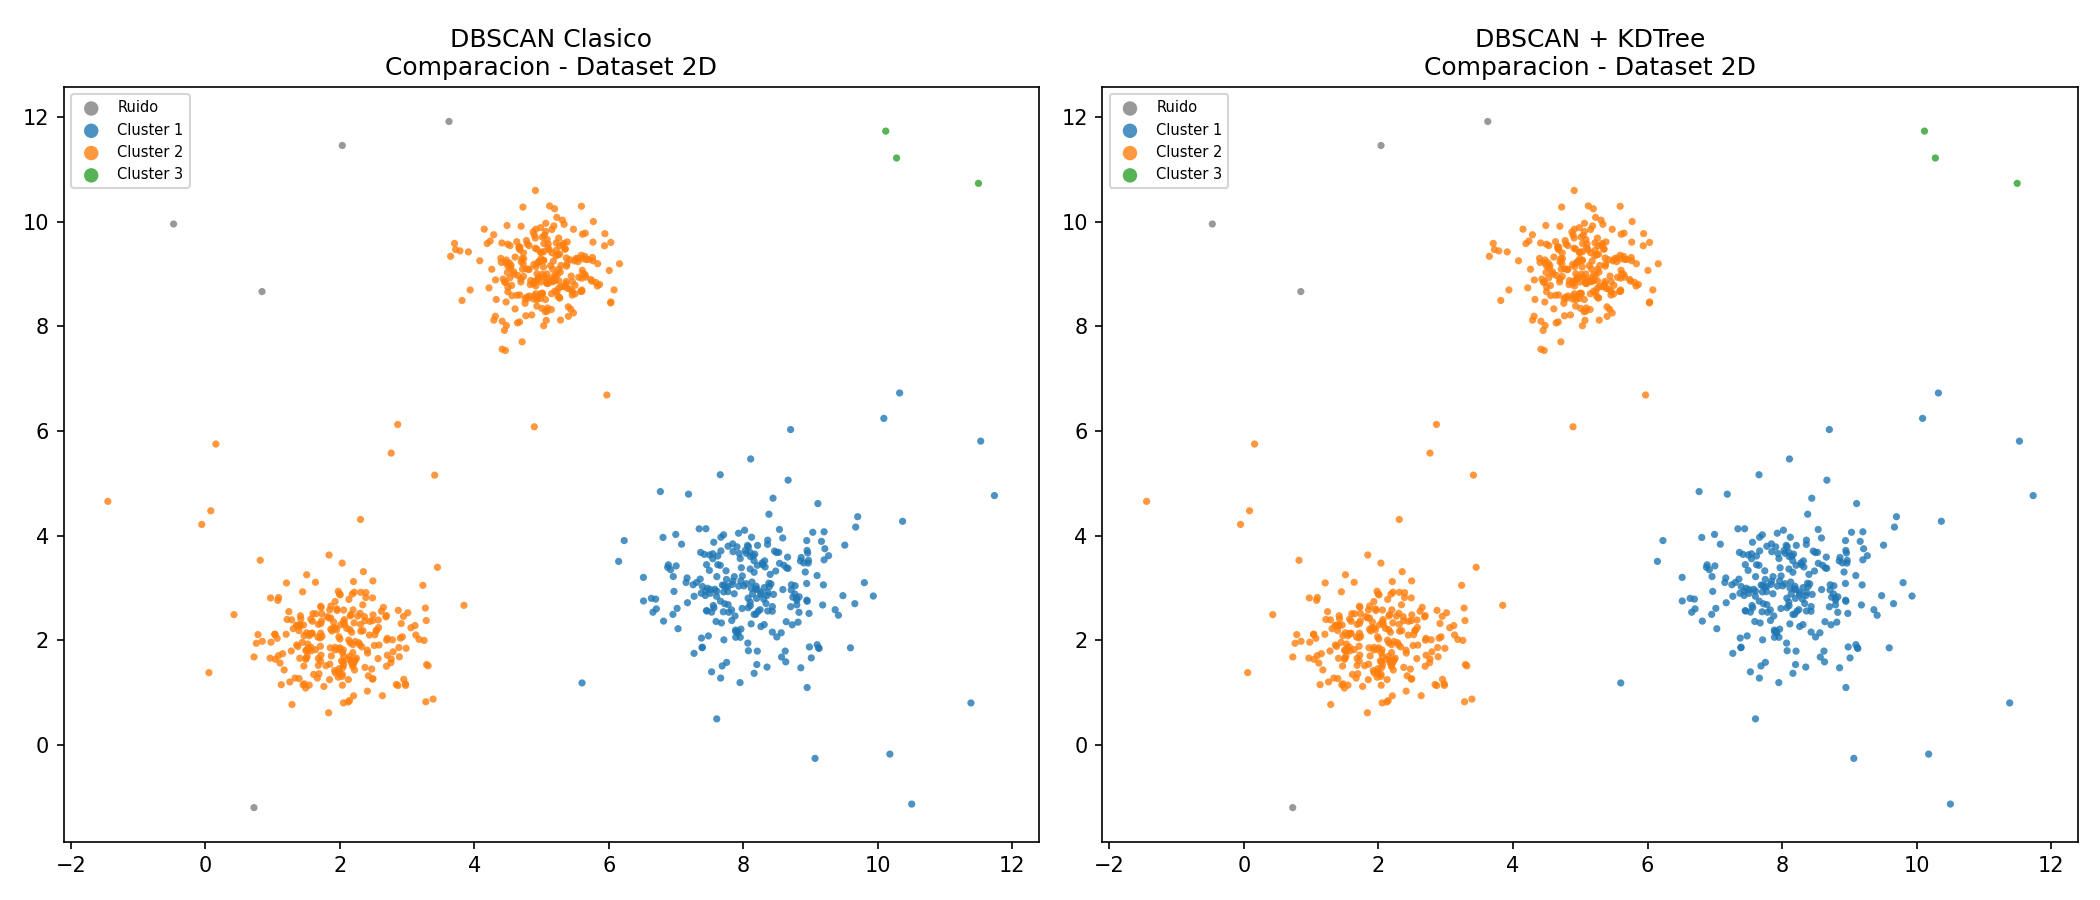
\includegraphics[width=\textwidth]{resultados/comparison_2d_2d_eps1.8_mp3.png}
    \caption{$\varepsilon=1.8$, minPts=3 (mayor cobertura)}
\end{subfigure}
\caption{Efecto de diferentes hiperparámetros en dataset 2D}
\end{figure}

Con $\varepsilon=1.2$ y minPts=3, el algoritmo encuentra 5 clusters (sobre-segmentación). Con $\varepsilon=1.8$ y minPts=3, solo 3 clusters pero con menos ruido (5 outliers vs 18-19).

\begin{figure}[H]
\centering
\begin{subfigure}{0.48\textwidth}
    \centering
    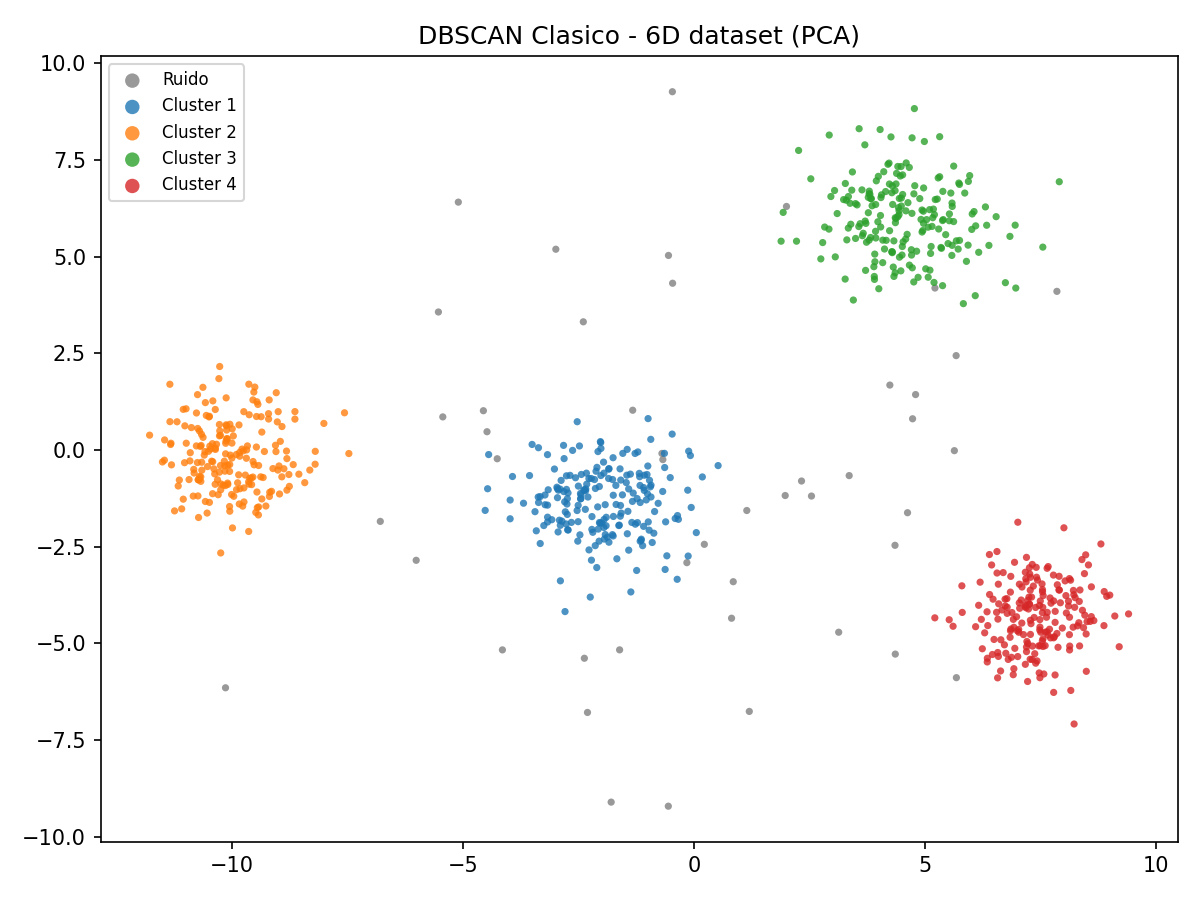
\includegraphics[width=\textwidth]{resultados/clusters_classic_6d_6d.png}
    \caption{Reducción PCA a 2D}
\end{subfigure}
\hfill
\begin{subfigure}{0.48\textwidth}
    \centering
    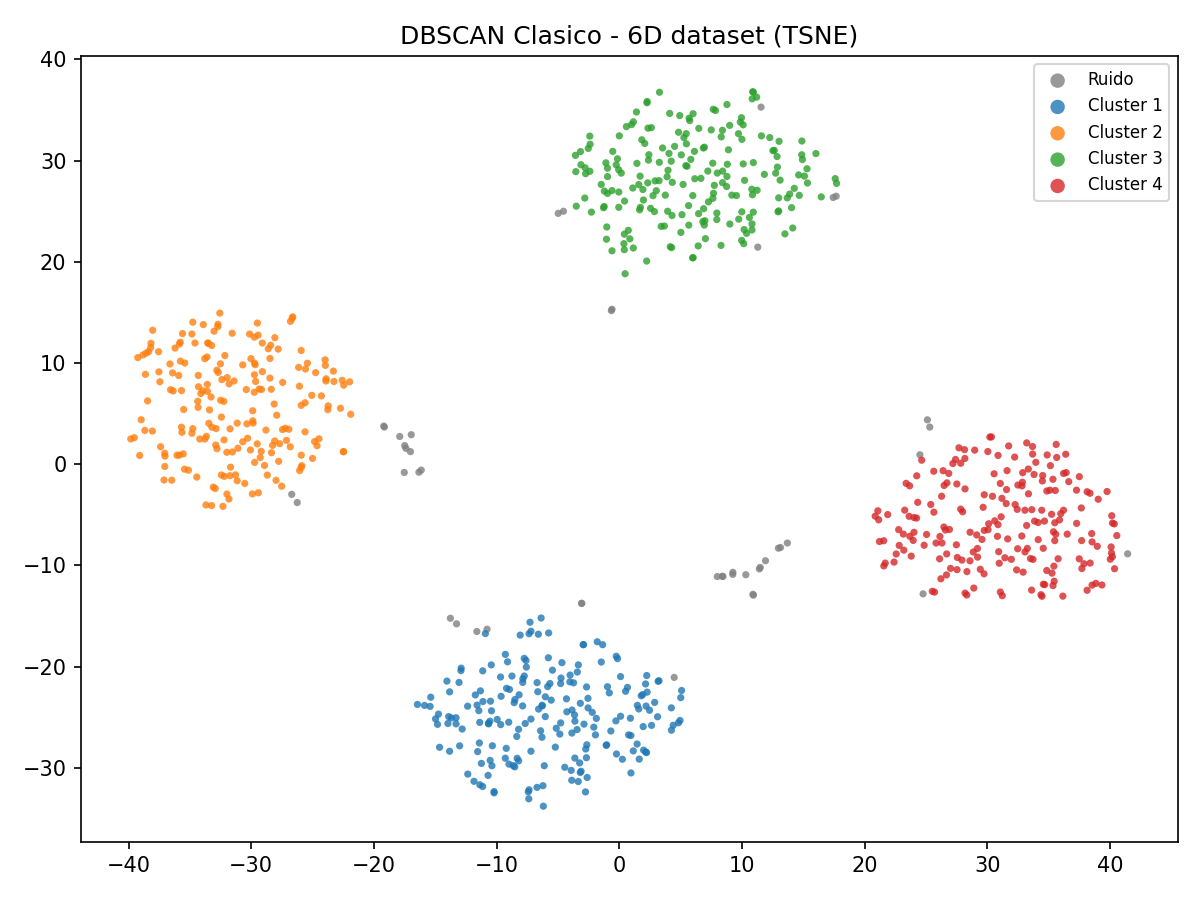
\includegraphics[width=\textwidth]{resultados/clusters_classic_6d_6d_tsne.png}
    \caption{Reducción t-SNE a 2D}
\end{subfigure}
\caption{Visualización del dataset 6D con reducción de dimensionalidad}
\end{figure}

\subsection{Métricas de Clustering}

\begin{table}[H]
\centering
\caption{Métricas de clustering para la configuración base}
\begin{tabular}{lcc}
\toprule
\textbf{Métrica} & \textbf{2D} & \textbf{6D} \\
\midrule
Puntos totales & 790 & 850 \\
Outliers & 19 & 46 \\
Clusters & 3 & 4 \\
Silhouette Score & 0.8181 & 0.7134 \\
\bottomrule
\end{tabular}
\end{table}

El Silhouette Score cercano a 1 indica clusters bien separados y cohesivos. El score en 2D (0.82) es excelente, mientras que en 6D (0.71) es bueno pero menor, reflejando la mayor dificultad de clustering en altas dimensiones.

% ========================
\section{Cuestionario}
% ========================

\subsection{Complejidad Computacional}

\textbf{DBSCAN Clásico:}
\begin{itemize}
    \item Búsqueda de vecinos: $O(n)$ por punto (fuerza bruta sobre todos los puntos).
    \item Total: $O(n^2)$ en el peor caso (cada punto visita todos los demás).
    \item Espacio: $O(n)$.
\end{itemize}

\textbf{DBSCAN + KDTree:}
\begin{itemize}
    \item Construcción del árbol: $O(n \log n)$.
    \item Búsqueda de vecinos por radio: $O(\log n)$ en promedio para $d$ baja.
    \item Total: $O(n \log n)$ promedio; $O(n^2)$ en el peor caso (árbol degenerado o dimensiones altas).
    \item Espacio: $O(n)$.
\end{itemize}

La complejidad del KDTree se degrada a $O(n)$ por búsqueda cuando la dimensionalidad es alta (``curse of dimensionality''), haciendo que la versión KDTree tienda a $O(n^2)$ en dimensiones $d > 20$.

\subsection{Estimación del Valor Inicial de \texttt{min\_samples}}

Una regla heurística común es:
\[
\texttt{min\_samples} \geq \text{dim} + 1
\]
Para datos de 2D, $\texttt{min\_samples} \geq 3$; para 6D, $\texttt{min\_samples} \geq 7$.

Otras estrategias incluyen:
\begin{itemize}
    \item Usar $\texttt{min\_samples} \approx 2 \cdot \text{dim}$ como punto de partida conservador.
    \item Para datasets grandes, valores entre 5 y 20 suelen ser razonables.
    \item Analizar el \textbf{k-distance graph}: graficar la distancia al $k$-ésimo vecino más cercano para cada punto (ordenado) y buscar el ``codo'' para estimar $\varepsilon$; min\_samples se fija como $k$.
\end{itemize}

\subsection{Estrategias para Optimizar \texttt{eps} y \texttt{min\_samples}}

\begin{enumerate}[label=\alph*)]
    \item \textbf{k-distance Graph:} Para un valor fijo de $k = \texttt{min\_samples}$, se calcula la distancia al $k$-ésimo vecino para cada punto y se ordena ascendentemente. El punto de máxima curvatura (codo) en esta gráfica sugiere un valor óptimo de $\varepsilon$.
    
    \item \textbf{Grid Search con Silhouette Score:} Probar combinaciones de $(\varepsilon, \texttt{min\_samples})$ en un rango y seleccionar la que maximice el Silhouette Score (o minimice el número de outliers con buen score).
    
    \item \textbf{Análisis de densidad local:} Estimar $\varepsilon$ como un percentil de las distancias $k$-NN (ej. percentil 90) para adaptarse a la densidad del dataset.
    
    \item \textbf{Conocimiento del dominio:} Si se conoce la escala de los datos o la distancia típica entre puntos del mismo cluster, $\varepsilon$ puede fijarse directamente.
\end{enumerate}

\subsection{Maldición de la Dimensionalidad y DBSCAN}

La ``maldición de la dimensionalidad'' afecta a DBSCAN de las siguientes maneras:

\begin{itemize}
    \item \textbf{Distancias menos significativas:} En altas dimensiones, las distancias entre puntos tienden a homogeneizarse (concentración de la medida). La diferencia entre el vecino más cercano y el más lejano se reduce, haciendo que el concepto de $\varepsilon$-vecindad pierda discriminación.
    
    \item \textbf{Densidad uniforme:} Los datos parecen distribuidos uniformemente en subespacios, dificultando la identificación de regiones densas.
    
    \item \textbf{Elección de $\varepsilon$:} Se requiere un $\varepsilon$ mayor para capturar suficientes vecinos, pero esto puede fusionar clusters distintos.
\end{itemize}

\textbf{Estrategias para manejar este problema:}
\begin{itemize}
    \item \textbf{Reducción de dimensionalidad} (PCA, t-SNE, UMAP) antes del clustering.
    \item \textbf{Selección de features} relevantes, eliminando dimensiones irrelevantes o redundantes.
    \item Usar métricas de distancia alternativas como \textbf{distancia coseno} o \textbf{Mahalanobis}.
    \item \textbf{Subespacios clustering:} Aplicar DBSCAN en subespacios proyectados de menor dimensión.
    \item Usar \textbf{OPTICS} (Ordering Points To Identify the Clustering Structure), que no requiere un $\varepsilon$ fijo y maneja mejor densidades variables.
\end{itemize}

\subsection{Limitaciones del KDTree en Alta Dimensionalidad y Alternativas}

\textbf{Limitaciones:}
\begin{itemize}
    \item La búsqueda por radio en KDTree se degrada de $O(\log n)$ a $O(n)$ cuando $d \gg \log_2 n$, porque el número de celdas intersectadas por la hiperesfera crece exponencialmente con $d$.
    \item En la práctica, para $d > 20$, la búsqueda secuencial puede ser más rápida que el KDTree.
    \item El árbol ocupa $O(n)$ en memoria pero con constantes altas por el almacenamiento de punteros.
\end{itemize}

\textbf{Alternativas:}
\begin{itemize}
    \item \textbf{Ball Tree:} Agrupa puntos en hiperesferas anidadas. Mejor adaptado a espacios métricos generales y sufre menos la maldición de la dimensionalidad que KDTree.
    \item \textbf{VP Tree (Vantage-Point Tree):} Útil para espacios métricos arbitrarios; particiona basándose en distancias a un punto de referencia.
    \item \textbf{LSH (Locality-Sensitive Hashing):} Usa funciones hash que preservan distancias para búsqueda aproximada de vecinos. Muy eficiente para alta dimensionalidad con búsqueda aproximada.
    \item \textbf{HNSW (Hierarchical Navigable Small World):} Estructura de grafo multicapa, estado del arte para búsqueda de vecinos en alta dimensionalidad (usado en ChromaDB, FAISS).
    \item \textbf{R-Tree / R*-Tree:} Índices espaciales jerárquicos con bounding boxes, eficientes para datos de baja a media dimensionalidad ($d \leq 10$).
    \item \textbf{Cover Tree:} Estructura teóricamente óptima para búsqueda por radio en espacios métricos de baja dimensión intrínseca.
\end{itemize}

% ========================
\section{Conclusiones}
% ========================

\begin{enumerate}
    \item La implementación de DBSCAN con KDTree ofrece una mejora de rendimiento del \textbf{25\%--36\%} respecto a la versión clásica en los datasets probados, reduciendo la complejidad de $O(n^2)$ a $O(n \log n)$ promedio.
    
    \item Ambas implementaciones producen \textbf{resultados idénticos} en términos de clusters y outliers, confirmando la corrección de la integración KDTree.
    
    \item El \textbf{Silhouette Score} (0.82 en 2D, 0.71 en 6D) demuestra que los clusters formados son cohesivos y bien separados.
    
    \item La elección de $\varepsilon$ y \texttt{min\_samples} es crítica: valores pequeños de $\varepsilon$ causan sobre-segmentación; valores grandes fusionan clusters distintos. El \textbf{k-distance graph} es la herramienta más recomendada para estimar $\varepsilon$.
    
    \item La \textbf{maldición de la dimensionalidad} afecta tanto a la calidad del clustering (distancias menos discriminativas) como a la eficiencia del KDTree (degradación de la búsqueda). Para $d > 20$, se recomiendan alternativas como Ball Tree, LSH o reducción de dimensionalidad previa.
    
    \item La combinación de \textbf{C++ para el cómputo intensivo} y \textbf{Python para visualización y métricas} resulta en una solución eficiente y flexible para el análisis de clustering.
\end{enumerate}

% ========================
\section{Anexo: Estructura del Código}
% ========================

El código fuente se organiza en los siguientes archivos:

\begin{itemize}
    \item \texttt{cpp/point.hpp} -- Estructura Point con coordenadas y etiqueta de cluster.
    \item \texttt{cpp/kdtree.hpp} -- Implementación header-only del KDTree con búsqueda por radio.
    \item \texttt{cpp/dbscan\_classic.cpp} -- DBSCAN con búsqueda de vecinos $O(n^2)$.
    \item \texttt{cpp/dbscan\_kdtree.cpp} -- DBSCAN optimizado con KDTree.
    \item \texttt{cpp/main.cpp} -- Programa principal: carga CSV, ejecuta ambos algoritmos, mide tiempos.
    \item \texttt{python/visualize.py} -- Visualización con matplotlib, PCA y t-SNE.
    \item \texttt{python/evaluate.py} -- Cálculo de métricas (Silhouette Score, outliers).
    \item \texttt{datasets/generate\_datasets.py} -- Generación de datasets sintéticos.
\end{itemize}

\textbf{Compilación y ejecución:}
\begin{lstlisting}[language=bash]
# Compilar
cd cpp && make

# Ejecutar
./dbscan ../datasets/2d_dataset.csv 1.5 5 2d
./dbscan ../datasets/nd_dataset.csv 4.0 10 6d

# Visualizar y evaluar
cd .. && python3 python/evaluate.py --classic resultados/2d_classic_labels.csv \
    --kdtree resultados/2d_kdtree_labels.csv --suffix 2d
python3 python/visualize.py --classic resultados/2d_classic_labels.csv \
    --kdtree resultados/2d_kdtree_labels.csv --suffix 2d
\end{lstlisting}

\end{document}
